\documentclass[tikz, border=10pt]{standalone}

% Required packages for drawing, colors, and fonts
\usepackage{tikz}
\usepackage{xcolor}
\usepackage{fontspec} % Use XeLaTeX or LuaLaTeX to compile

% TikZ libraries for positioning nodes, arrow styles, shadings, and decorations
\usetikzlibrary{positioning, arrows.meta, shadings, decorations.pathreplacing}

% Set a sans-serif font similar to the one in the image (e.g., Helvetica/Arial)
% TeX Gyre Heros is a good open-source alternative.
\setsansfont{TeX Gyre Heros}

% --- Custom Color Definitions ---
% Define colors that closely match the image
\definecolor{bgcolor}{HTML}{F0F3F8}
% Gradient for Conv/Concat blocks
\definecolor{grad1_left}{HTML}{DDC8FF} 
\definecolor{grad1_right}{HTML}{FFB3A7}
% Gradient for PSABlock blocks
\definecolor{grad2_left}{HTML}{A440B2}
\definecolor{grad2_right}{HTML}{FF8C82}

\begin{document}

% Set the background color for the entire image
\pagecolor{bgcolor}

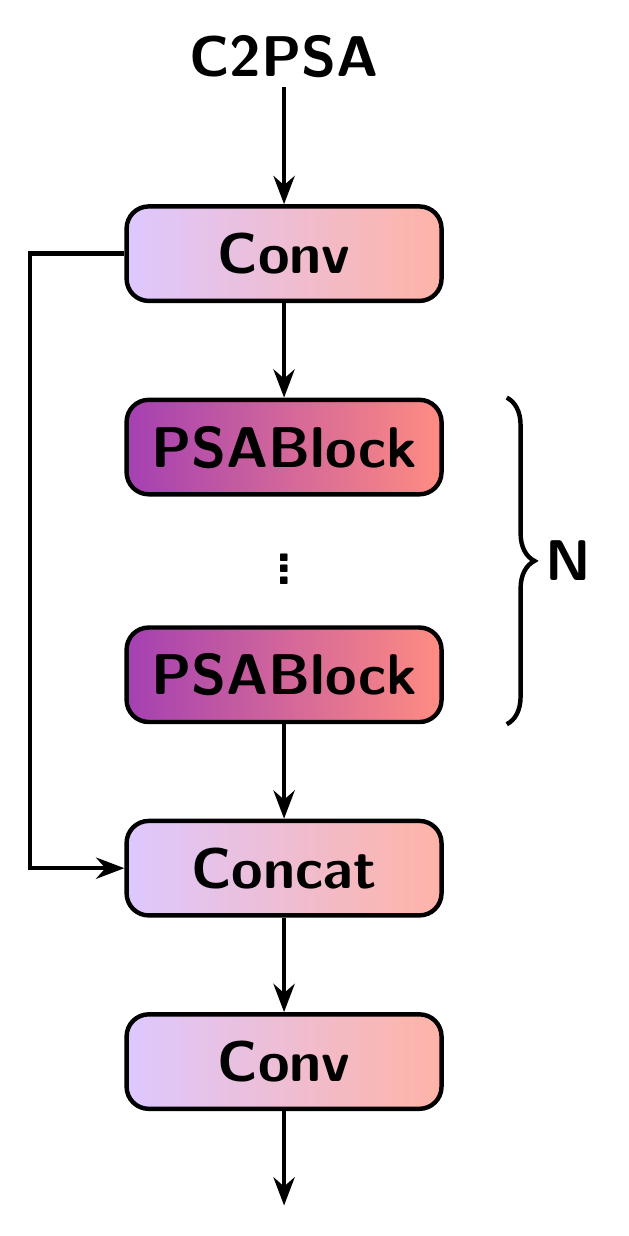
\begin{tikzpicture}[
    % --- Global Settings ---
    % Set default node distance for vertical spacing
    node distance = 1.2cm,
    % Set font for all nodes in the picture
    every node/.style={font=\sffamily\bfseries\huge}
  ]

  % --- Style Definitions ---
  % Style for the main blocks (rounded corners, thick border, size, and font)
  \tikzset{
    block/.style={
      draw=black, 
      ultra thick, 
      rounded corners=8pt, 
      minimum width=4cm, 
      minimum height=1.2cm,
      align=center
    },
    % Style for the first type of gradient (blue/purple to red/pink)
    gradient1/.style={
      left color=grad1_left, 
      right color=grad1_right
    },
    % Style for the second type of gradient (deep purple to red)
    gradient2/.style={
      left color=grad2_left, 
      right color=grad2_right
    },
    % Style for the arrows (thick, black, with a specific arrowhead)
    arrow/.style={
      ->, 
      ultra thick, 
      >=Stealth
    }
  }

  % --- Node Placement ---
  % Place all nodes, starting from the top and working downwards.
  % The 'positioning' library is used to place nodes relative to each other.
  
  % Input label node
  \node (c2psa) at (0, 8.5) {C2PSA};

  % First convolutional block
  \node[block, gradient1] (conv1) at (0, 6) {Conv};

  % First PSA block
  \node[block, gradient2] (psa1) [below=of conv1] {PSABlock};

  % Ellipsis indicating repetition
  \node (dots) [below=0.4cm of psa1] {\vdots};

  % Second PSA block
  \node[block, gradient2] (psa2) [below=0.4cm of dots] {PSABlock};

  % Concatenation block
  \node[block, gradient1] (concat) [below=of psa2] {Concat};

  % Second convolutional block
  \node[block, gradient1] (conv2) [below=of concat] {Conv};

  % --- Path and Arrow Drawing ---
  % Draw all the connections between the nodes.
  
  % Main vertical flow
  \draw[arrow] (c2psa.south) -- (conv1.north);
  \draw[arrow] (conv1.south) -- (psa1.north);
  % The flow between psa1, dots, and psa2 is implied.
  \draw[arrow] (psa2.south) -- (concat.north);
  \draw[arrow] (concat.south) -- (conv2.north);
  % Final output arrow
  \draw[arrow] (conv2.south) -- ++(0,-1.2);

  % Skip connection path from the first Conv to Concat
  % The path starts at conv1.west, moves left, turns down, and goes into concat.west
  \draw[arrow] (conv1.west) -- ++(-1.2,0) |- (concat.west);

  % --- Brace and Label ---
  % Draw the brace on the right side to indicate N blocks.
  \draw[
    decoration={brace, amplitude=10pt}, % Use the brace decoration
    decorate,                           % Apply the decoration
    ultra thick                         % Make the brace thick
  ] 
  ([xshift=0.8cm]psa1.north east) -- ([xshift=0.8cm]psa2.south east) % Brace coordinates
  node[midway, right=10pt] {N}; % Place the 'N' label to the right of the brace's midpoint

\end{tikzpicture}

\end{document}